% Options for packages loaded elsewhere
\PassOptionsToPackage{unicode}{hyperref}
\PassOptionsToPackage{hyphens}{url}
%
\documentclass[
]{book}
\usepackage{amsmath,amssymb}
\usepackage{lmodern}
\usepackage{iftex}
\ifPDFTeX
  \usepackage[T1]{fontenc}
  \usepackage[utf8]{inputenc}
  \usepackage{textcomp} % provide euro and other symbols
\else % if luatex or xetex
  \usepackage{unicode-math}
  \defaultfontfeatures{Scale=MatchLowercase}
  \defaultfontfeatures[\rmfamily]{Ligatures=TeX,Scale=1}
\fi
% Use upquote if available, for straight quotes in verbatim environments
\IfFileExists{upquote.sty}{\usepackage{upquote}}{}
\IfFileExists{microtype.sty}{% use microtype if available
  \usepackage[]{microtype}
  \UseMicrotypeSet[protrusion]{basicmath} % disable protrusion for tt fonts
}{}
\makeatletter
\@ifundefined{KOMAClassName}{% if non-KOMA class
  \IfFileExists{parskip.sty}{%
    \usepackage{parskip}
  }{% else
    \setlength{\parindent}{0pt}
    \setlength{\parskip}{6pt plus 2pt minus 1pt}}
}{% if KOMA class
  \KOMAoptions{parskip=half}}
\makeatother
\usepackage{xcolor}
\usepackage{longtable,booktabs,array}
\usepackage{calc} % for calculating minipage widths
% Correct order of tables after \paragraph or \subparagraph
\usepackage{etoolbox}
\makeatletter
\patchcmd\longtable{\par}{\if@noskipsec\mbox{}\fi\par}{}{}
\makeatother
% Allow footnotes in longtable head/foot
\IfFileExists{footnotehyper.sty}{\usepackage{footnotehyper}}{\usepackage{footnote}}
\makesavenoteenv{longtable}
\usepackage{graphicx}
\makeatletter
\def\maxwidth{\ifdim\Gin@nat@width>\linewidth\linewidth\else\Gin@nat@width\fi}
\def\maxheight{\ifdim\Gin@nat@height>\textheight\textheight\else\Gin@nat@height\fi}
\makeatother
% Scale images if necessary, so that they will not overflow the page
% margins by default, and it is still possible to overwrite the defaults
% using explicit options in \includegraphics[width, height, ...]{}
\setkeys{Gin}{width=\maxwidth,height=\maxheight,keepaspectratio}
% Set default figure placement to htbp
\makeatletter
\def\fps@figure{htbp}
\makeatother
\usepackage[normalem]{ulem}
\setlength{\emergencystretch}{3em} % prevent overfull lines
\providecommand{\tightlist}{%
  \setlength{\itemsep}{0pt}\setlength{\parskip}{0pt}}
\setcounter{secnumdepth}{5}
\usepackage{booktabs}
\AtBeginDocument{\renewcommand{\chaptername}{}}  


\usepackage{booktabs}
\usepackage{longtable}
\usepackage{array}
\usepackage{multirow}
\usepackage{wrapfig}
\usepackage{float}
\usepackage{colortbl}
\usepackage{pdflscape}
\usepackage{tabu}
\usepackage{threeparttable}
\usepackage{threeparttablex}
\usepackage[normalem]{ulem}
\usepackage{makecell}
\usepackage{xcolor}
\ifLuaTeX
  \usepackage{selnolig}  % disable illegal ligatures
\fi
\usepackage[]{natbib}
\bibliographystyle{apalike}
\IfFileExists{bookmark.sty}{\usepackage{bookmark}}{\usepackage{hyperref}}
\IfFileExists{xurl.sty}{\usepackage{xurl}}{} % add URL line breaks if available
\urlstyle{same} % disable monospaced font for URLs
\hypersetup{
  pdftitle={TEXT BOOK OF AGRICULTURAL STATISTICS},
  pdfauthor={Dr.~Pratheesh P. Gopinath},
  hidelinks,
  pdfcreator={LaTeX via pandoc}}

\title{TEXT BOOK OF AGRICULTURAL STATISTICS}
\author{Dr.~Pratheesh P. Gopinath}
\date{}

\begin{document}
\maketitle

{
\setcounter{tocdepth}{1}
\tableofcontents
}
\hypertarget{textbook-of-agricultural-statistics}{%
\chapter*{Textbook of Agricultural Statistics}\label{textbook-of-agricultural-statistics}}

\hypertarget{dedication}{%
\section*{Dedication}\label{dedication}}

To my beloved wife, Saliny S Nair, who has always been my source of inspiration and unwavering support throughout my journey. Your love, encouragement, and understanding have been instrumental in making this book a reality.

To my dear children, Aadiseshan and Anandapadmanabhan, who fill my life with joy and laughter. You are my motivation to keep learning and growing every day.

To my parents, whose unwavering love and support have been the foundation of my life. Your guidance and encouragement have shaped me into the person I am today, and I am forever grateful.

This book is dedicated to all of you with love and gratitude.

~

Copyright © 2023 by Pratheesh P Gopinath

All rights reserved. No part of this book may be reproduced in any form or by any means, electronic or mechanical, including photocopying, recording, or by any information storage and retrieval system, without permission in writing from the author, except by a reviewer who may quote brief passages in a review.

ISBN: 9798840789896

Imprint: Independently published

KINDLE DIRECT PUBLISHING

Cover design by Pratheesh P Gopinath

For information on permissions, translation rights, or bulk purchases, please contact \texttt{pratheesh@kaugrapes.com}

\hypertarget{preface}{%
\chapter*{Preface}\label{preface}}
\addcontentsline{toc}{chapter}{Preface}

Agricultural statistics is a crucial field of study for students pursuing undergraduate programs in agriculture. However, the subject is often perceived as complex and challenging, and students may find it difficult to comprehend the basic concepts and principles.

In addition, statistics is also important in agricultural research for making informed decisions based on the results of experiments and surveys. By using statistical methods to analyze data, researchers can draw conclusions about the effectiveness of different agricultural practices, the impact of environmental factors on crop yields, and the efficacy of new technologies in agriculture. Furthermore, statistics is crucial in ensuring the accuracy and validity of research findings, and helps to prevent biased or misleading interpretations of data. As such, a strong understanding of statistical principles and techniques is essential for any student or professional working in the field of agriculture.

As a result, I wrote this book, ``Text book of Agricultural Statistics,'' to provide a comprehensive and accessible introduction to the subject. This book is written with the objective of helping students, who are beginners in statistics, understand the fundamental concepts and principles of agricultural statistics with ease.

The book covers a wide range of topics, from basic statistical concepts such as probability theory and data presentation to advanced techniques like regression analysis and experimental designs. Each topic is explained in a clear and concise manner, with examples and illustrations provided to help the reader understand the concepts in a practical context.

Throughout the book, I have tried to use simple language and minimize technical jargon to ensure that the content is accessible to readers who have no prior experience with statistics. The examples used are drawn from the field of agriculture, making the book more relevant and engaging for students in this field.

I hope that this book will serve as a useful resource for students pursuing undergraduate programs in agriculture, as well as for professionals who wish to refresh their knowledge of agricultural statistics. I also believe that this book will help readers develop an appreciation for the role of statistics in the field of agriculture, and inspire them to apply statistical techniques to solve real-world problems in this field.

I would like to express my gratitude to all those who supported me throughout the writing of this book. I would also like to acknowledge the valuable feedback and suggestions provided by colleagues and students, which have helped to improve the content of this book.

Finally, I would like to encourage readers to provide feedback on this book, as I believe that this will help me to improve the content and make future editions even more useful to readers. Write me to \texttt{pratheesh@kaugrapes.com}

Thank you,

Dr Pratheesh P Gopinath

\hypertarget{introduction}{%
\chapter{Introduction}\label{introduction}}

In this chapter, we will explore the fundamentals of statistics, including its definition, history, and contributions, as well as some basic concepts that are essential for understanding statistical science.

The history of statistics can be traced back to ancient civilizations, such as the Babylonians, who used statistics for agricultural purposes, and the Egyptians, who used it for census purposes. However, it wasn't until the 17th century that statistics began to emerge as a formal field of study, thanks to the work of prominent mathematicians such as John Graunt, William Petty, and Blaise Pascal.

Over the years, statistics has evolved into a multidisciplinary field that draws upon various disciplines, such as mathematics, probability theory, and computer science. It has made significant contributions to fields such as epidemiology, psychology, engineering, and finance, among others.

To understand statistics, one needs to have a good grasp of some basic concepts. These concepts provide a foundation for more advanced statistical techniques.

In the following sections, we will delve deeper into these concepts and explore how they are used in statistical analysis. We will also examine some common applications of statistics and discuss how they have contributed to the advancement of various fields. By the end of this chapter, you should have a solid understanding of the basics of statistics and be ready to explore more advanced statistical techniques\citep{goon} \citep{gupta}

\hypertarget{origin-of-the-word-statistics}{%
\section{Origin of the word ``Statistics''}\label{origin-of-the-word-statistics}}

The term statistics was derived from the Neo-Latin word
\texttt{statisticum\ collegium} meaning ``council of state'' and the Italian word
\texttt{statista} meaning ``statesman'' or ``politician''.

A German word \texttt{Statistik}, got the meaning ``collection and
classification of data'' generally in the early 19th century. This word
was first introduced by Gottfried Achenwall (1749). \texttt{Statistik} was
originally designated as a term for analysis of data about the state
(data used by government or other administrative bodies). The term
\texttt{Statistik} was introduced into English in 1791 by Sir John Sinclair
when he published the first of 21 volumes titled ``Statistical Account of
Scotland'' \citep{ball}. The first book to have `Statistics' in its title was
``Contributions to Vital Statistics'' (1845) by Francis GP Neison,
actuary\footnote{actuary: A person who compiles and analyses
  statistics and uses them to calculate insurance risks and premiums.} to the Medical Invalid and General Life Office.

\begin{figure}

{\centering 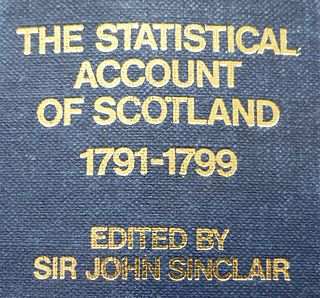
\includegraphics[width=4.44in]{images/history1} 

}

\caption{Statistical Account of Scotland by Sir John Sinclair (1791)}\label{fig:scotland}
\end{figure}

\hypertarget{statistics-and-mathematics}{%
\section{Statistics and Mathematics}\label{statistics-and-mathematics}}

Mathematics follows a rigid theorem and proof. Mathematical theories
involve well-defined and proven facts which has the minimal scope of
change. However, Statistics is a discipline where real-life data is
handled. This factor makes this field of study more abstract, where
individuals have to develop newer solutions to problems that was new and
not observed before. Statistics is an applied science; in mathematics
the goal is to prove theorems. In statistics, the main goal is to
develop good methods for understanding data and making decisions.
Statisticians often use mathematical theorems to justify their methods,
but theorems are not the main focus. Statistics is now considered as an
independent field which uses mathematics to solve real life problems.

In terms of error, mathematics and statistics differ in how they handle and approach errors.

Mathematics is all about getting the right answer. It focuses on using formulas and equations to solve problems accurately, and mistakes are considered human errors that can be corrected.

Statistics, on the other hand, acknowledges that there will always be some errors when collecting and analyzing data. Instead of trying to avoid errors altogether, statisticians use different techniques to measure and control them. They try to get the best possible estimate of the true values of the data and take into account the uncertainty and potential errors associated with those estimates.

In summary, mathematics is concerned with minimizing errors in the application of mathematical principles and calculations, while statistics acknowledges the presence of errors in data and aims to quantify and control them through statistical techniques.

\hypertarget{definition-of-statistics}{%
\section{Definition of Statistics}\label{definition-of-statistics}}

Statistics is the science which deals with the

\begin{itemize}
\item
  Collection of data
\item
  Organization of data or Classification of data
\item
  Presentation of data
\item
  Analysis of data
\item
  Interpretation of data
\end{itemize}

Two main branches of statistics are:

\textbf{Descriptive statistics}, is a branch of statistics that involves summarizing and presenting data in a meaningful way. It is used to describe and understand the features of a data set by providing numerical or graphical summaries of the data.

Descriptive statistics is a way to summarize and present data in a useful way. It can be used to describe things like the average score of a class or how spread out the scores are. for example such measures will help the teachers and administrators understand how well students are doing and identify areas where they need to improve.

\textbf{Inferential statistics}, uses a small group of data called a random sample to make predictions or draw conclusions about a larger group called the population. The goal is to learn about the characteristics, or parameters, of the population by analyzing the data from the sample. In other words, we use the data we have from a smaller group to make educated guesses about the characteristics of a larger group.

For example, imagine you want to know the average height of all students in a school, but it would take too much time and effort to measure the height of every student. Instead, you can take a sample of students and measure their height. By using inferential statistics, you can estimate the average height of all students in the school based on the height measurements of the sample.

Inferential statistics uses probability theory and statistical techniques to make inferences about a population based on the characteristics of a sample. It allows researchers to test hypotheses and make predictions with a certain level of confidence based on the data available.

Descriptive statistics is used to summarize and present data in a meaningful way, while inferential statistics is used to make predictions or draw conclusions about a larger group based on a smaller sample. Descriptive statistics provides a summary of the data that is easy to understand and use, while inferential statistics allows us to make generalizations about a larger population based on the characteristics of a smaller sample.

\hypertarget{father-of-statistics}{%
\section{Father of Statistics}\label{father-of-statistics}}

Ronald Aylmer Fisher (R.A. Fisher) is often referred to as the ``father of statistics'' because of his numerous contributions to statistical theory and methodology. He developed several statistical tests and methods that are still widely used today, such as analysis of variance (ANOVA) and maximum likelihood estimation.

Prasanta Chandra Mahalanobis (P.C. Mahalanobis), on the other hand, is regarded as the ``father of Indian statistics'' because of his pioneering work in developing statistical methods that were specifically suited to the unique challenges of the Indian context. He founded the Indian Statistical Institute and developed the Mahalanobis distance, which is still used in fields such as image recognition and pattern analysis. He also played a key role in shaping India's national statistical system and promoting the use of statistics in policymaking.

\hypertarget{scope-of-statistics}{%
\section{Scope of statistics}\label{scope-of-statistics}}

\textbf{Functions of statistics}: Statistics simplifies complexity, presents
facts in a definite form, helps in formulation of suitable policies,
facilitates comparison and helps in forecasting. Valid results and
conclusion are obtained in research experiments using proper statistical
tools.

\begin{itemize}
\item
  Summarize data: Statistics can be used to take large amounts of data and present it in a simple and understandable way.
\item
  Analyze data: Statistics can be used to identify patterns, trends, and relationships in data, which can help us to understand various phenomena.
\item
  Make decisions: Statistics can be used to provide accurate and reliable information that can be used to support decision-making processes.
\item
  Test hypotheses: Statistics can be used to test theories or ideas by analyzing data and drawing conclusions based on the results.
\item
  Estimate parameters: Statistics can be used to estimate characteristics of a larger group, called the population, based on information collected from a smaller group, called the sample.
\item
  Model relationships: Statistics can be used to create models that show how different variables are related to one another, which can be used to make predictions and inform future decisions.
\end{itemize}

Overall, statistics helps us to make sense of the world by providing tools to organize and analyze data, and to draw meaningful conclusions from it.

\textbf{Uses of statistics:} Statistics has pervaded almost all spheres of
human activities. Statistics is useful in the administration, Industry,
business, economics, research workers, banking,insurance companies etc.

\begin{itemize}
\item
  Business: Statistics can be used to analyze sales data, customer behavior, and market trends to help businesses make informed decisions about pricing, product development, and marketing strategies.
\item
  Healthcare: Statistics can be used to analyze patient data, evaluate the effectiveness of treatments, and identify risk factors for various diseases.\\
\item
  Science: Statistics can be used to design experiments, analyze data from experiments, and make predictions based on data.
\item
  Government: Statistics can be used to gather information about populations, monitor trends in crime, and evaluate the effectiveness of public policies.
\item
  Education: Statistics can be used to evaluate student performance, develop educational programs, and measure the effectiveness of teaching methods.
\item
  Sports: Statistics can be used to analyze player performance, evaluate team strategies, and predict the outcome of games.
\end{itemize}

Overall, statistics plays an important role in helping us to make informed decisions and understand the world around us.

\hypertarget{the-architects-of-statistical-theory}{%
\section{The Architects of Statistical Theory}\label{the-architects-of-statistical-theory}}

Statistics is a field that has a long history of important contributors who have made significant contributions to the development of statistical theory and practice. There have been many prominent statisticians throughout history, including several notable Indian statisticians who have made significant contributions to the field. Here are a few of the most important statisticians throughout history:

\textbf{Ronald Aylmer Fisher}: R. A. Fisher was an English statistician and geneticist who is widely considered to be one of the founders of modern statistics. He made significant contributions to statistical theory, including the development of methods for analyzing variance, the design of experiments, and the development of maximum likelihood estimation. Fisher was also a pioneer in the field of genetics, and his work on the inheritance of traits has had a lasting impact on the field.

\textbf{Karl Pearson}: Pearson was an English mathematician and statistician who is best known for his work on correlation and regression analysis. He also made significant contributions to the development of the chi-squared test, which is widely used in statistical hypothesis testing.

\textbf{William S. Gosset}: Gosset, who is also known by his pen name ``Student,'' was an English statistician who worked for the Guinness Brewery in Dublin, Ireland. He developed the t-test, which is used to determine whether the means of two groups are significantly different from one another. Gosset's work on the t-test had a significant impact on the development of statistical inference.

\textbf{Florence Nightingale}: Nightingale was an English nurse who is widely considered to be the founder of modern nursing. She also made significant contributions to the field of statistics, particularly in the area of medical statistics. Nightingale used statistical methods to analyze data on mortality rates and other health-related data, and her work had a significant impact on the development of public health policies.

\textbf{Sir David Cox}: Cox is an English statistician who is best known for his work on survival analysis and the development of the proportional hazards model. He also made significant contributions to the development of methods for analyzing categorical data and the analysis of variance. Cox's work has had a significant impact on many fields, including medicine, epidemiology, and engineering.

\textbf{P.C.Mahalanobis}: Prasanta Chandra Mahalanobis was an Indian statistician who is best known for his work on multivariate analysis and the development of the Mahalanobis distance. He was the founder of the Indian Statistical Institute, which he established in 1931 with the goal of advancing statistical research and training in India. Mahalanobis was also instrumental in the development of the National Sample Survey, which has been used to collect data on a wide range of topics in India since the 1950s.

\textbf{C.R. Rao}: Calyampudi Radhakrishna Rao is another prominent Indian statistician who has made significant contributions to the field. He is known for his work on statistical theory, matrix algebra, and multivariate analysis. Rao has received numerous awards for his contributions to statistics, including the National Medal of Science in the United States and the Royal Society's Copley Medal. C.R. Rao has earned a reputation as a living legend in the field. In 2023, Rao was awarded the International Prize in Statistics, an award often touted as the ``statistics' equivalent of the Nobel Prize''.

\textbf{Ramanujan}: While not traditionally thought of as a statistician, Srinivasa Ramanujan was a mathematician who made significant contributions to the field of number theory. His work on the partition function, which counts the number of ways that a positive integer can be expressed as a sum of other positive integers, has applications in statistical mechanics and the analysis of algorithms. Ramanujan's contributions to mathematics and statistics have had a lasting impact on the field.

\textbf{Bhattacharya}: Subhashis Bhattacharya is a contemporary Indian statistician who is known for his work on probability theory and stochastic processes. He has received numerous awards for his contributions to the field, including the Shanti Swarup Bhatnagar Prize in Mathematical Sciences, which is one of the highest scientific honors in India.

\textbf{Basu}: Pranab Kumar Basu is another prominent Indian statistician who has made significant contributions to the field. He is known for his work on survey sampling, statistical inference, and Bayesian analysis. Basu has received numerous awards for his contributions to statistics, including the Padma Shri award, which is one of the highest civilian honors in India.

These are just a few examples of statisticians who have made significant contributions to the field. Their work has helped to advance statistical theory and practice, and has had a lasting impact on the way that we collect, analyze, and interpret data.

\hypertarget{agricultural-statistics-in-india}{%
\section{Agricultural Statistics in India}\label{agricultural-statistics-in-india}}

Agriculture is a vital sector in India's economy, contributing approximately 16\% of the country's GDP and employing over 50\% of the population. As such, agricultural statistics play a crucial role in monitoring and evaluating the performance of the sector.

The Indian agricultural statistical system comprises several institutions, including the Ministry of Agriculture and Farmers Welfare, the Department of Agriculture, Cooperation and Farmers Welfare, and the Directorate of Economics and Statistics. These institutions are responsible for collecting, compiling, and analyzing data related to agriculture, including crop production, livestock, land use, irrigation, and agricultural finance.

One of the main sources of agricultural statistics in India is the Agricultural Census. Conducted every five years, this census collects data on various aspects of agriculture, such as land use, irrigation, livestock, and crop production. The data collected in the Agricultural Census provides a comprehensive picture of the state of agriculture in the country and helps policymakers to make informed decisions.

In addition to the Agricultural Census, several surveys are also conducted to collect data on specific aspects of agriculture, such as the National Sample Survey (NSS) on Household Consumption Expenditure, which collects data on agricultural household income and expenditure patterns, and the Annual Report on the Price Situation of Agricultural Commodities, which monitors prices of agricultural commodities.

Agricultural statistics in India also play an essential role in international trade. India is one of the world's largest exporters of agricultural products, such as rice, wheat, and cotton. The collection and analysis of agricultural statistics help policymakers to monitor the performance of the sector, identify areas for improvement, and make informed decisions about trade policies.

In conclusion, agricultural statistics in India play a crucial role in monitoring and evaluating the performance of the agricultural sector. The data collected and analyzed helps policymakers to make informed decisions about policies related to agriculture, including crop production, livestock, land use, irrigation, and agricultural finance. By providing a comprehensive picture of the state of agriculture in the country, agricultural statistics play an essential role in supporting the growth and development of the sector.

\hypertarget{some-basic-concepts}{%
\chapter{Some basic concepts}\label{some-basic-concepts}}

Statistics is all about making sense of data, and to do that effectively, you need to understand some fundamental concepts. In this chapter, we will explore some basic concepts in statistics that are essential for anyone who wants to analyze data.

\hypertarget{population-and-sample}{%
\section{Population and Sample}\label{population-and-sample}}

Consider the following example.Suppose we wish to study the body masses
of all students of College of Agriculture, Vellayani. It will take us a
long time to measure the body masses of all students of the college and
so we may select 20 of the students and measure their body masses (in
kg). Suppose we obtain the measurements like this

49 56 48 61 59 43 58 52 64 71 57 52 63 58 51 47 57 46 53 59

In this study, we are interested in the body masses of all students of
College of Agriculture, Vellayani. The set of body masses of all
students of College of Agriculture, Vellayani is called the
\textbf{population} of this study. The set of 20 body masses, \emph{W} = \{49,
56,48, \ldots, 53, 59\}, is a \textbf{sample} from this population.

\hypertarget{population}{%
\subsection{Population}\label{population}}

A population is the set of all objects we wish to study.

In statistics, a population refers to the entire group of individuals, objects, or events that we are interested in studying. It is the entire set of units or elements that share one or more characteristics of interest to the researcher. The population can be of any size, depending on the research question and the resources available to the researcher.

For example, if a researcher is interested in studying the attitudes of all the farmers in a village, the population would be all the farmers in that village. If a researcher is interested in studying the prevalence of a disease in cattle in a particular area only, the population would be all the cattle in that area.

It is important to define the population clearly, as it forms the basis for sampling and making inferences about the larger group.

\hypertarget{sample}{%
\subsection{Sample}\label{sample}}

A sample is part of the population we study to learn about the
population.

In statistics, a sample is a subset of a population that is selected for study. The purpose of taking a sample is to study a smaller group of individuals, objects, or events from the larger population, and to use the information obtained from the sample to make inferences about the population as a whole.

Sampling is a crucial part of statistical analysis, as it allows researchers to study a population without having to study every individual, which can be time-consuming and costly. The sample should be selected in a way that is representative of the population of interest, so that the results of the study can be generalized to the larger population.

The size of the sample also plays an important role in determining the accuracy of the estimates. Generally, the larger the sample size, the more accurate the estimates are likely to be.

\hypertarget{variables-and-constants}{%
\section{Variables and constants}\label{variables-and-constants}}

\hypertarget{variables}{%
\subsection{Variables}\label{variables}}

Any type of observation which can take different values for different
people, or different values at different times, or places, is called a
variable. The following are examples of variables:

\begin{itemize}
\item
  family size, number of hospital beds, number of schools in a
  country, etc.
\item
  height, mass, blood pressure, temperature, blood glucose level, etc.
\end{itemize}

Broadly speaking, there are two types of variables -- \textbf{quantitative}
and \textbf{qualitative} (or categorical) variables

\hypertarget{constants}{%
\subsection{Constants}\label{constants}}

Constants are characteristics that have values that do not change.
Examples of constants are: pi (\(\pi\)) = the ratio of the circumference of a
circle to its diameter (\(\pi\) = 3.14159...) and \emph{e}, the base of the
natural or (Napierian) logarithms (\emph{e}=2.71828).

\hypertarget{types-of-variables}{%
\section{Types of variables}\label{types-of-variables}}

\hypertarget{quantitative-variables}{%
\subsection{Quantitative variables}\label{quantitative-variables}}

A quantitative variable is one that can take numerical values. The
variables like family size, number of hospital beds, number of schools
in a country, height, mass, blood pressure, temperature, blood glucose
level, etc. are examples of quantitative variables. Quantitative
variables may be characterized further as to whether they are discrete
or continuous

\hypertarget{discrete-variables}{%
\subsection{Discrete variables}\label{discrete-variables}}

The variables like family size, number of hospital beds, number of
schools in a country, etc. can be counted. These are examples of
discrete variables. Variables that can only take on a finite number of
values are called ``discrete variables.'' Any variable phrased as ``the
number of \ldots{}'', is discrete, because it is possible to list its possible
values \{0,1, \ldots\}. Any variable with a finite number of possible values
is discrete. The following example illustrates the point. The number of
daily admissions to a hospital is a discrete variable since it can be
represented by a whole number, such as 0, 1, 2 or 3. The number of daily
admissions on a given day cannot be a number such as 1.8, 3.96 or 5.33.

\hypertarget{continuous-variables}{%
\subsection{Continuous variables}\label{continuous-variables}}

The variables like height, mass, blood pressure, temperature, blood
glucose level, etc. can be measured. These are examples of continuous
variables. A continuous variable does not possess the gaps or
interruptions characteristic of a discrete variable. A continuous
variable can assume any value within a specific relevant interval of
values assumed by the variable. Notice that age is continuous since an
individual does not age in discrete jumps. Weight can be measured as
35.5, 35.8 kg etc so, it is a continuous variable.

\hypertarget{categorical-variables}{%
\subsection{Categorical variables}\label{categorical-variables}}

A variable is called categorical when the measurement scale is a set of
categories. For example, marital status, with categories
(single,married, widowed), is categorical. Whether employed (yes, no),
religious affiliation (Protestant, Catholic, Jewish, Muslim, others,
none), colours etc. Categorical variables are often called qualitative.
It can be seen that categorical variables can neither be measured nor
counted.

\hypertarget{measurement-scales}{%
\section{Measurement scales}\label{measurement-scales}}

Variables can further be classified according to the following four
levels of measurement: nominal, ordinal, interval and ratio.

\hypertarget{nominal-scale}{%
\subsection{Nominal scale}\label{nominal-scale}}

This scale of measure applies to qualitative variables only. On the
nominal scale, no order is required. For example,gender is nominal,
blood group is nominal, and marital status is also nominal. We cannot
perform arithmetic operations on data measured on the nominal scale.

\hypertarget{ordinal-scale}{%
\subsection{Ordinal scale}\label{ordinal-scale}}

This scale also applies to qualitative data. On the ordinal scale, order
is necessary. This means that one category is lower than the next one or
vice versa. For example, Grades are ordinal, as excellent is higher than
very good, which in turn is higher than good, and so on. It should be
noted that, in the ordinal scale, differences between category values
have no meaning.

\hypertarget{interval-scale}{%
\subsection{Interval scale}\label{interval-scale}}

This scale of measurement applies to quantitative data only. In this
scale, the zero point does not indicate a total absence of the quantity
being measured. An example of such a scale is temperature on the Celsius
or Fahrenheit scale. Suppose the minimum temperatures of 3 cities, A, B
and C, on a particular day were 0\textsuperscript{0}C, 20\textsuperscript{0}C and 10\textsuperscript{0}C, respectively.
It is clear that we can find the differences between these temperatures.
For example, city B is 20\textsuperscript{0}C hotter than city A. However, we cannot say
that city A has no temperature. Moreover, we cannot say that city B is
twice as hot as city C, just because city B is 20\textsuperscript{0}C and city C is
10\textsuperscript{0}C. The reason is that, in the interval scale, the ratio between two
numbers is not meaningful.

\hypertarget{ratio-scale}{%
\subsection{Ratio scale}\label{ratio-scale}}

This scale of measurement also applies to quantitative data only and has
all the properties of the interval scale. In addition to these
properties, the ratio scale has a meaningful zero starting point and a
meaningful ratio between 2 numbers. An example of variables measured on
the ratio scale, is weight. A weighing scale that reads 0 kg gives an
indication that there is absolutely no weight on it. So the zero
starting point is meaningful. If Ram weighs 40 kg and Laxman weighs 20
kg, then Ram weighs twice as Laxman. Another example of a variable
measured on the ratio scale is temperature measured on the Kelvin scale.
This has a true zero point.

\begin{figure}

{\centering 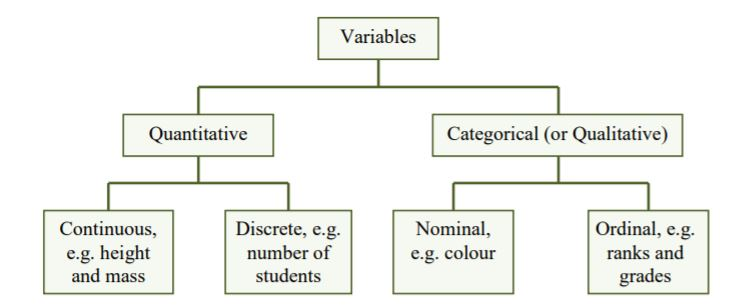
\includegraphics[width=0.7\linewidth]{images/image2} 

}

\caption{Classification of variables}\label{fig:variables}
\end{figure}

\hypertarget{data}{%
\section{Data}\label{data}}

Data can be defined as individual pieces of factual information recorded
and used for the purpose of analysis. It is the raw information from
which inferences are drawn using the science ``STATISTICS''.

Data refers to information that is collected and recorded for analysis. This information can be in the form of numbers, text, images, or other formats and can be obtained from a variety of sources. The analysis of data can help to identify patterns, trends, and relationships, and can be used to inform decision making in many different fields.

Example for data

\begin{itemize}
\item
  No.~of farmers in a block.
\item
  The rainfall over a period of time.
\item
  Area under paddy crop in a state.
\item
  Images of rice blast disease
\end{itemize}

\hypertarget{collection-of-data}{%
\section{Collection of Data}\label{collection-of-data}}

The first step in any enquiry (investigation) is the collection of data.
The data may be collected for the whole population or for a sample only.
It is mostly collected on a sample basis. Collecting data is very
difficult job. The enumerator or investigator is the well trained
individual who collects the statistical data. The respondents are the
persons from whom the information is collected.

\hypertarget{types-of-data}{%
\subsection{Types of Data}\label{types-of-data}}

There are two types (sources) for the collection of data:\\
* Primary Data

\begin{itemize}
\tightlist
\item
  Secondary Data
\end{itemize}

\hypertarget{primary-data}{%
\subsubsection{Primary Data}\label{primary-data}}

Primary data are the first hand information which is collected, compiled
and published by organizations for some purpose. They are the most
original data in character and have not undergone any sort of
statistical treatment.

Example: Population census reports are primary data because these are
collected, complied and published by the population census organization.

\hypertarget{secondary-data}{%
\subsubsection{Secondary Data}\label{secondary-data}}

The secondary data are the second hand information which is already
collected by an organization for some purpose and are available for the
present study. Secondary data are not pure in character and have
undergone some treatment at least once.

Example: An economic survey of England is secondary data because the
data are collected by more than one organization like the Bureau of
Statistics, Board of Revenue, banks, etc.

\hypertarget{methods-of-collecting-primary-data}{%
\section{Methods of Collecting Primary Data}\label{methods-of-collecting-primary-data}}

Primary data are collected using the following methods:

\hypertarget{personal-investigation}{%
\subsection{Personal Investigation}\label{personal-investigation}}

The researcher conducts the survey him/herself and collects data from
it. The data collected in this way are usually accurate and reliable.
This method of collecting data is only applicable in case of small
research projects.

\hypertarget{through-investigation}{%
\subsection{Through Investigation}\label{through-investigation}}

Trained investigators are employed to collect the data. These
investigators contact the individuals and fill in questionnaires after
asking for the required information. Most organizations utilize this
method.

\hypertarget{collection-through-questionnaire}{%
\subsection{Collection through Questionnaire}\label{collection-through-questionnaire}}

Researchers get the data from local representations or agents that are
based upon their own experience. This method is quick but gives only a
rough estimate.

\hypertarget{through-the-telephone}{%
\subsection{Through the Telephone}\label{through-the-telephone}}

Researchers get information from individuals through the telephone. This
method is quick and gives accurate information.

\hypertarget{methods-of-collecting-secondary-data}{%
\section{Methods of Collecting Secondary Data}\label{methods-of-collecting-secondary-data}}

Secondary data are collected by the following methods:

\hypertarget{official}{%
\subsection{Official}\label{official}}

Publications from the Statistical Division, Ministry of Finance, the
Federal Bureaus of Statistics, Ministries of Food, Agriculture,
Industry, Labor, etc.

\hypertarget{semi-official}{%
\subsection{Semi-Official}\label{semi-official}}

\begin{itemize}
\tightlist
\item
  Publications from State Bank, Railway Board, Central Cotton
  Committee, Boards of Economic Enquiry etc.\\
\item
  Publication of Trade Associations, Chambers of Commerce, etc.\\
\item
  Technical and Trade Journals and Newspapers.\\
\item
  Research Organizations such as universities and other institutions.
\end{itemize}

\hypertarget{difference-between-primary-and-secondary-data}{%
\section{Difference Between Primary and Secondary Data}\label{difference-between-primary-and-secondary-data}}

The difference between primary and secondary data is only a change of
hand. Primary data are the first hand information which is directly
collected form one source. They are the most original in character and
have not undergone any sort of statistical treatment, while secondary
data are obtained from other sources or agencies. They are not pure in
character and have undergone some treatment at least once.

\hypertarget{self-evaluation-quiz}{%
\section{Self-Evaluation Quiz}\label{self-evaluation-quiz}}

\hypertarget{fill-in-the-blanks}{%
\section*{Fill in the blanks}\label{fill-in-the-blanks}}

\begin{enumerate}
\def\labelenumi{\arabic{enumi}.}
\item
  \_\_\_\_\_\_\_\_\_\_ is a complete set of individuals, objects, or
  measurements of interest.
\item
  \_\_\_\_\_\_\_\_\_\_ is a subset of a population, selected for study
  in some prescribed manner.
\item
  \_\_\_\_\_\_\_\_\_\_ is a characteristic of interest that varies
  from one individual, object, or measurement to another.
\item
  \_\_\_\_\_\_\_\_\_\_ is a characteristic of interest that remains
  constant for all individuals, objects, or measurements in a study.
\item
  \_\_\_\_\_\_\_\_\_\_ is the process of collecting information from
  individuals, objects, or measurements of interest.
\item
  \_\_\_\_\_\_\_\_\_\_ data are collected by the investigator for the
  first time, while \_\_\_\_\_\_\_\_\_\_ data are obtained from a
  third-party source.
\item
  \_\_\_\_\_\_\_\_\_\_ variable is one whose values are determined by
  chance.
\item
  \_\_\_\_\_\_\_\_\_\_ variable is one whose values depend on or are
  determined by the values of another variable.
\item
  On a \_\_\_\_\_\_\_\_\_\_ scale, both the order and the distance
  between values are meaningful.
\item
  An example of a variable measured on an \_\_\_\_\_\_\_\_\_\_ scale
  is temperature in degrees Celsius or Fahrenheit.
\item
  A \_\_\_\_\_\_\_\_\_\_ scale has a true zero point, meaning that a
  value of zero indicates the complete absence of the characteristic
  being measured.
\item
  An example of a variable measured on a \_\_\_\_\_\_\_\_\_\_ scale is
  weight in kilograms or pounds.
\item
  On a \_\_\_\_\_\_\_\_\_\_ scale, the order of values is meaningful,
  but the distance between values is not.
\item
  An example of a variable measured on an \_\_\_\_\_\_\_\_\_\_ scale
  is socioeconomic status, as measured by income level.
\item
  The \_\_\_\_\_\_\_\_\_\_ is the ratio of the distance between two
  values on a measurement scale to the difference between the
  corresponding values.
\item
  The \_\_\_\_\_\_\_\_\_\_ of a measurement scale refers to the range
  of values that can be measured on the scale.
\item
  In statistical analysis, variables measured on \_\_\_\_\_\_\_\_\_\_
  scales often allow for more powerful analyses and more meaningful
  conclusions.
\item
  One important consideration when choosing a measurement scale is the
  level of \_\_\_\_\_\_\_\_\_\_ required by the research question or
  hypothesis being tested.
\item
  Temperature measured in Kelvin is in \_\_\_\_\_\_\_\_\_\_ scale.
\item
  \_\_\_\_\_\_\_ refers to any collection of facts, numbers, or other
  information that can be analyzed to gain knowledge or make
  decisions.
\end{enumerate}

\begin{quote}
\textbf{Answers}: 1. population, 2. sample, 3. variable, 4. constant, 5. data collection, 6. primary, secondary, 7. random, 8. dependent, 9. interval, 10. interval, 11. ratio, 12. ratio, 13. ordinal, 14. ordinal, 15. scale factor, 16. range, 17. interval or ratio, 18. precision, 19. ratio, 20. data
\end{quote}

\hypertarget{multiple-choice-questions}{%
\section*{Multiple choice questions}\label{multiple-choice-questions}}

\begin{enumerate}
\def\labelenumi{\arabic{enumi}.}
\item
  Which of the following is an example of a variable?

  \begin{enumerate}
  \def\labelenumii{\alph{enumii}.}
  \item
    A rock
  \item
    The color blue
  \item
    Age
  \item
    All of the above
  \end{enumerate}
\item
  What is the difference between a population and a sample?

  \begin{enumerate}
  \def\labelenumii{\alph{enumii}.}
  \item
    A population is a subset of a sample.
  \item
    A sample is a subset of a population.
  \item
    A population and a sample are the same thing.
  \item
    A population is larger than a sample.
  \end{enumerate}
\item
  Which of the following is an example of a ratio scale measurement?

  \begin{enumerate}
  \def\labelenumii{\alph{enumii}.}
  \item
    The rating of a restaurant on a scale from 1 to 5 stars
  \item
    The level of education completed by a person (e.g., high school,
    college, graduate degree)
  \item
    The number of hours worked in a week
  \item
    The weight of a person in kilograms or pounds
  \end{enumerate}
\item
  What is the difference between primary and secondary data?

  \begin{enumerate}
  \def\labelenumii{\alph{enumii}.}
  \item
    Primary data are collected by the investigator, while secondary
    data are obtained from a third-party source.
  \item
    Primary data are obtained from a third-party source, while
    secondary data are collected by the investigator.
  \item
    Primary data and secondary data are the same thing.
  \item
    Primary data are more reliable than secondary data.
  \end{enumerate}
\item
  Which of the following is an example of an ordinal scale
  measurement?

  \begin{enumerate}
  \def\labelenumii{\alph{enumii}.}
  \item
    Height in centimeters
  \item
    Number of siblings
  \item
    Rank of preference for different ice cream flavors
  \item
    Number of pets
  \end{enumerate}
\item
  What is the primary characteristic of a nominal scale measurement?

  \begin{enumerate}
  \def\labelenumii{\alph{enumii}.}
  \item
    It has an arbitrary zero point.
  \item
    It is used for ranking and ordering data.
  \item
    It uses numerical values to represent quantities.
  \item
    It categorizes data into mutually exclusive and exhaustive
    categories.
  \end{enumerate}
\item
  Which of the following is an example of a variable measured on an
  interval scale?

  \begin{enumerate}
  \def\labelenumii{\alph{enumii}.}
  \item
    The weight of a person in pounds
  \item
    The type of car a person drives
  \item
    The score on a multiple choice exam
  \item
    The level of agreement on a Likert scale survey question
  \end{enumerate}
\item
  What is the main difference between a ratio scale measurement and an
  interval scale measurement?

  \begin{enumerate}
  \def\labelenumii{\alph{enumii}.}
  \item
    A ratio scale measurement has an arbitrary zero point, while an
    interval scale measurement does not.
  \item
    An interval scale measurement is used to measure non-numeric
    variables, while a ratio scale measurement is used to measure
    numeric variables.
  \item
    A ratio scale measurement can have a value of zero, while an
    interval scale measurement cannot.
  \item
    An interval scale measurement is less precise than a ratio scale
    measurement.
  \end{enumerate}
\item
  Which of the following is an example of a categorical variable?

  \begin{enumerate}
  \def\labelenumii{\alph{enumii}.}
  \item
    Age
  \item
    Weight
  \item
    Gender
  \item
    Temperature in Celsius
  \end{enumerate}
\item
  Which of the following is an example of a continuous variable?

  \begin{enumerate}
  \def\labelenumii{\alph{enumii}.}
  \item
    Number of pets
  \item
    Blood type
  \item
    Number of siblings
  \item
    Height in centimeters
  \end{enumerate}

  \textbf{Answers}
\end{enumerate}

\begin{longtable}[]{@{}
  >{\raggedright\arraybackslash}p{(\columnwidth - 18\tabcolsep) * \real{0.0976}}
  >{\raggedright\arraybackslash}p{(\columnwidth - 18\tabcolsep) * \real{0.0976}}
  >{\raggedright\arraybackslash}p{(\columnwidth - 18\tabcolsep) * \real{0.0976}}
  >{\raggedright\arraybackslash}p{(\columnwidth - 18\tabcolsep) * \real{0.0976}}
  >{\raggedright\arraybackslash}p{(\columnwidth - 18\tabcolsep) * \real{0.0976}}
  >{\raggedright\arraybackslash}p{(\columnwidth - 18\tabcolsep) * \real{0.0976}}
  >{\raggedright\arraybackslash}p{(\columnwidth - 18\tabcolsep) * \real{0.0976}}
  >{\raggedright\arraybackslash}p{(\columnwidth - 18\tabcolsep) * \real{0.0976}}
  >{\raggedright\arraybackslash}p{(\columnwidth - 18\tabcolsep) * \real{0.0976}}
  >{\raggedright\arraybackslash}p{(\columnwidth - 18\tabcolsep) * \real{0.0976}}@{}}
\toprule()
\begin{minipage}[b]{\linewidth}\raggedright
1
\end{minipage} & \begin{minipage}[b]{\linewidth}\raggedright
2
\end{minipage} & \begin{minipage}[b]{\linewidth}\raggedright
3
\end{minipage} & \begin{minipage}[b]{\linewidth}\raggedright
4
\end{minipage} & \begin{minipage}[b]{\linewidth}\raggedright
5
\end{minipage} & \begin{minipage}[b]{\linewidth}\raggedright
6
\end{minipage} & \begin{minipage}[b]{\linewidth}\raggedright
7
\end{minipage} & \begin{minipage}[b]{\linewidth}\raggedright
8
\end{minipage} & \begin{minipage}[b]{\linewidth}\raggedright
9
\end{minipage} & \begin{minipage}[b]{\linewidth}\raggedright
10
\end{minipage} \\
\midrule()
\endhead
\textbf{c} & \textbf{b} & \textbf{d} & \textbf{a} & \textbf{c} & \textbf{d} & \textbf{d} & \textbf{c} & \textbf{c} & d \\
\bottomrule()
\end{longtable}

\hypertarget{frequency-distribution}{%
\chapter{Frequency distribution}\label{frequency-distribution}}

Frequency distribution is an essential tool in statistics that summarizes the distribution of a dataset by showing how often each value occurs. A frequency distribution provides a visual representation of the data that allows for easy interpretation and analysis. Example below will help you understand more about frequency distribution.

Table shows the number of children per family for 54 families selected
from a town in India. The data, presented in this form in which it was
collected, is called raw data.

\begin{figure}

{\centering 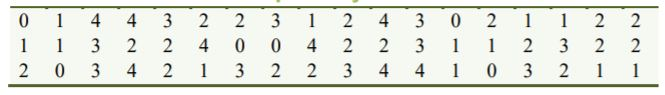
\includegraphics[width=0.7\linewidth]{images/image3} 

}

\caption{raw data set of No. of children in 54 families}\label{fig:raw}
\end{figure}

It can be seen that, the minimum and the maximum numbers of children per
family are 0 and 4, respectively. Apart from these numbers, it is
impossible, without further careful study, to extract any exact
information from the data. But by breaking down the data into the form
below

\begin{figure}

{\centering 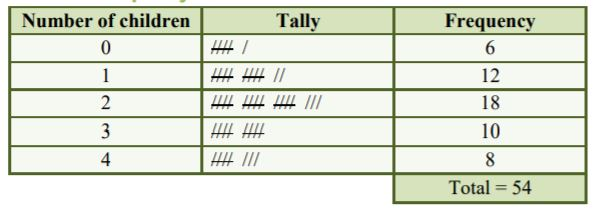
\includegraphics[width=0.9\linewidth]{images/image4} 

}

\caption{Frequency distribution table}\label{fig:freq}
\end{figure}

Now certain features of the data become apparent. For instance, it can
easily be seen that, most of the 54 families selected have two children
because number of houses having 2 children is 18. This information
cannot easily be obtained from the raw data. The above table is called a
frequency table or a frequency distribution. It is so called because it
gives the frequency or number of times each observation occurs. Thus, by
finding the frequency of each observation, a more intelligible picture
is obtained.

\hypertarget{construction-of-frequency-distribution}{%
\subsection{Construction of frequency distribution}\label{construction-of-frequency-distribution}}

\begin{enumerate}
\def\labelenumi{\arabic{enumi}.}
\item
  List all values of the variable in ascending order of magnitude.
\item
  Form a tally column, that is, for each value in the data, record a
  stroke in the tally column next to that value. In the tally, each
  fifth stroke is made across the first four. This makes it easy to
  count the entries and enter the frequency of each observation.
\item
  Check that the frequencies sum to the total number of observations
\end{enumerate}

\hypertarget{grouped-frequency-distribution}{%
\section{Grouped frequency distribution}\label{grouped-frequency-distribution}}

Data below gives the body masses of 22 patients, measured to the nearest
kilogram.

\begin{figure}

{\centering 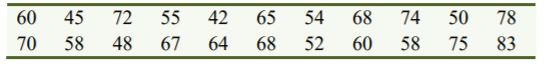
\includegraphics[width=0.9\linewidth]{images/image5} 

}

\caption{Body masses of 22 patients}\label{fig:mass}
\end{figure}

It can be seen that the minimum and the maximum body masses are 42 kg
and 83 kg, respectively. A frequency distribution giving every body mass
between 42 kg and 83 kg would be very long and would not be very
informative. The problem is to overcome by grouping the data into
classes.\\
If we choose the classes\\
41 -- 49\\
50 -- 58\\
59 -- 67\\
68 -- 76 and 77 -- 85, we obtain the frequency distribution given below:

\begin{figure}

{\centering 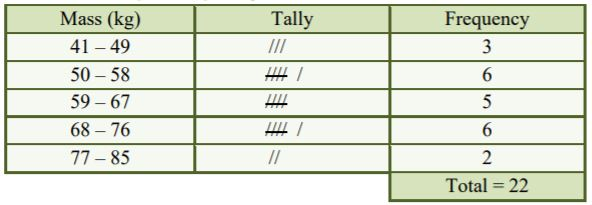
\includegraphics[width=0.9\linewidth]{images/image6} 

}

\caption{Grouped Frequency distribution table}\label{fig:grptable}
\end{figure}

Above table gives the frequency of each group or class; it is therefore
called a grouped frequency table or a grouped frequency distribution.
Using this grouped frequency distribution, it is easier to obtain
information about the data than using the raw data. For instance, it can
be seen that 17 of the 22 patients have body masses between 50 kg and 76
kg (both inclusive). This information cannot easily be obtained from the
raw data.\\
It should be noted that, even though above table is concise, some
information is lost. For example, the grouped frequency distribution
does not give us the exact body masses of the patients. Thus the
individual body masses of the patients are lost in our effort to obtain
an overall picture.

\hypertarget{terms-used-in-grouped-frequency-tables.}{%
\section{Terms used in grouped frequency tables.}\label{terms-used-in-grouped-frequency-tables.}}

\textbf{Class limits}

The intervals into which the observations are put are called \uline{class
intervals}. The end points of the class intervals are called
\uline{class limits}. For example, the class interval 41 -- 49,
has lower class limit 41 and upper class limit 49.

\textbf{Class boundaries}

The raw data in the above example were recorded to the nearest kilogram.
Thus, a body mass of 49.5kg would have been recorded as 50 kg, a body
mass of 58.4 kg would have been recorded as 58 kg, while a body mass of
58.5 kg would have been recorded as 59 kg. It can therefore be seen
that, the class interval 50 -- 58, consists of measurements greater than
or equal to 49.5 kg and less than 58.5 kg. The numbers 49.5 and 58.5 are
called the lower and upper boundaries of the class interval 50 -- 58.
The class boundaries of the other class intervals are given below:

\begin{figure}

{\centering 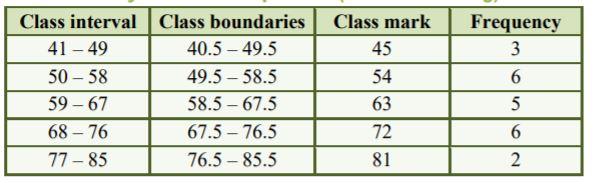
\includegraphics[width=0.9\linewidth]{images/image7} 

}

\caption{Class boundary and class limits}\label{fig:clsslmt}
\end{figure}

\uline{Note:}\\
Notice that the lower class boundary of the i\textsuperscript{th} class interval is the
mean of the lower class limit of the class interval and the upper class
limit of the (i-1)\textsuperscript{th} class interval (i = 2, 3, 4, \ldots). For example,
in the table above the lower class boundaries of the second and the
fourth class intervals are (50 + 49) /2 = 49.5 and (68 + 67)/2 = 67.5
respectively.\\
It can also be seen that the upper class boundary of the i\textsuperscript{th} class
interval is the mean of the upper class limit of the class interval and
the lower class limit of the (i+1)\textsuperscript{th} class interval (i = 1, 2, 3,
\ldots). Thus, in the above table the upper class boundary of the fourth
class interval is (76 + 77)/2 = 76.5.

\textbf{Class mark}\\
The mid-point of a class interval is called the class mark or class
mid-point of the class interval. It is the average of the upper and
lower class limits of the class interval. It is also the average of the
upper and lower class boundaries of the class interval. For example, in
the table, the class mark of the third class interval was found as
follows: class mark =(59+67) /2 = (58.5 + 67.5)/2= 63.

\textbf{Class width}\\
The difference between the upper and lower class boundaries of a class
interval is called the class width of the class interval. Class widths
of class intervals can also be found by subtracting two consecutive
lower class limits, or by subtracting two consecutive upper class
limits.

\uline{Note:}

The width of the i\textsuperscript{th} class interval is the numerical difference
between the upper class limits of the i\textsuperscript{th} and the ( i-1)\textsuperscript{th} class
intervals (i = 2, 3, \ldots). It is also the numerical difference between
the lower class limits of the i\textsuperscript{th} and the (i+1) \textsuperscript{th} class intervals
(i = 1, 2, \ldots).

In grouped frequency table above the width of the first class interval
is \textbar41-50\textbar{} = 9. This is the numerical difference between the lower
class limits of the first and the second class intervals. The width of
the second class interval is \textbar50-59\textbar= 9. This is the numerical
difference between the lower class limits of the second and the third
class intervals. It is also equal to \textbar58-49\textbar{} the numerical, difference
between the upper class limits of the first and the second class
intervals.

\hypertarget{construction-of-frequency-distribution-table}{%
\section{Construction of frequency distribution table}\label{construction-of-frequency-distribution-table}}

\textbf{Step 1}. Decide how many classes you wish to use.\\
\textbf{Step 2}. Determine the class width\\
\textbf{Step 3}. Set up the individual class limits\\
\textbf{Step 4}. Tally the
items into the classes\\
\textbf{Step 5}. Count the number of items in each class

I will explain the construction process with the example below:

\begin{quote}
An agricultural student measured the lengths of leaves on an oak tree (to the nearest cm). Measurements on 38 leaves are as follows
\end{quote}

\begin{quote}
9,16,13,7,8,4,18,10,17,18,9,12,5,9,9,16,1,8,17,1,10,5,9,11,15,6,14,9,1,12,5,16,4,16,8,15,14,17
\end{quote}

\textbf{Step 1.} Decide how many classes you wish to use.

H.A. Sturges provides a formula for determining the approximation number
of classes.\\
\[\mathbf{k^{'} = 1 + 3.322}\mathbf{\log}\mathbf{N}\]\\
If \(k^{'}\) is a decimal value, then the Number of classes (\emph{k}) is obtained by rounding \(k^{'}\) to the nearest higher integer.

If \(k^{'}\) is an integer,the number of classes (\emph{k}) is equal to \(k^{'}\).

In our example \emph{N}=38, so \(k^{'}\)=1+3.322×log(38) = 1+3.322×1.5797 = 6.24\\
here \(k^{'}\) is a decimal value so it is rounded to next higher integer, that is 7

So the number of classes (\emph{k}) = 7

\textbf{Step 2.} Determine the class width (\emph{C})

Generally, the class width should be the same size for all classes. Formula for calculating approximate number of classes is\\
\[C^{'} = {| max -min|\over k^{'}}\]\\
Note that \(k^{'}\) used here is the approximation number of classes using Struges formula not the rounded number of class (\emph{k}).

If \(C^{'}\) is a decimal value, then the class width (\emph{C}) is obtained by rounding \(C^{'}\) to the nearest higher integer.

If \(C^{'}\) is an integer,the class width (\emph{C}) is equal to \(C^{'}\).

For this example, \(C^{'}\) = \textbar{} 18− 1\textbar/\textbf{6.24} = 2.72, here \(C^{'}\) is a decimal value so it is rounded to next higher integer, that is 3. so class width \emph{C} = 3.

\textbf{Step 3.} To set up the individual class limits, We need to find the
lower limit only

\[L = min - \frac{C \times k - (max - min)}{2}\]

where \emph{C} and \emph{k} here are class width and number of classes respectively in our example

\(L = 1 - \frac{3 \times 7 - (18 - 1)}{2}\)=1-2= -1; since there is no
negative values in data = 0.

\begin{table}[H]
\centering
\begin{tabular}[t]{cc}
\toprule
Class & Frequency\\
\midrule
0-3 & 3\\
3-6 & 5\\
6-9 & 5\\
9-12 & 9\\
12-15 & 5\\
\addlinespace
15-18 & 9\\
18-21 & 2\\
\bottomrule
\end{tabular}
\end{table}

Even though the student only measured in whole numbers, the data is
continuous, so ``4 cm'' means the actual value could have been anywhere
from 3.5 cm to 4.5 cm.

\hypertarget{cumulative-frequency}{%
\section{Cumulative frequency}\label{cumulative-frequency}}

In many situations, we are not interested in the number of observations
in a given class interval, but in the number of observations which are
less than (or greater than) a specified value. For example, in the above
table, it can be seen that 3 leaves have length less than 3.5 cm and 9
leaves (i.e.~3 + 6) have length less than 6.5 cm. These frequencies are
called cumulative frequencies. A table of such cumulative frequencies is
called \textbf{a cumulative frequency table} or \textbf{cumulative frequency
distribution}.

Cumulative frequency is defined as a running total of frequencies.
Cumulative frequency can also defined as the sum of all previous
frequencies up to the current point. Notice that the last cumulative
frequency is equal to the sum of all the frequencies. Two types of
cumulative frequencies are Less than cumulative frequency and Greater
than cumulative frequency. Less than cumulative frequency (LCF) is the
number of values less than a specified value. Greater than cumulative
frequency (GCF) is the number of observations greater than a specified
value.

The specified value for LCF in the case of grouped frequency
distribution will be upper limits and for GCF will be the lower limits
of the classes. LCF's are obtained by adding frequencies in the
successive classes and GCF are obtained by subtracting the successive
class frequencies from the total frequency.

\hypertarget{relative-frequency}{%
\section{Relative frequency}\label{relative-frequency}}

It is sometimes useful to know the proportion, rather than the number,
of values falling within a particular class interval. We obtain this
information by dividing the frequency of the particular class interval
by the total number of observations. \textbf{Relative frequency} of a class
is the frequency of class / total observation. Relative frequencies all
add up to 1.

\begin{table}[H]
\centering
\begin{tabular}[t]{ccccc}
\toprule
Class & Frequency & A & B & C\\
\midrule
0.5 - 3.5 & 3 & 3 & 38 & 0.078947\\
3.5 - 6.5 & 6 & 9 & 35 & 0.157895\\
6.5 - 9.5 & 10 & 19 & 29 & 0.263158\\
9.5 -12.5 & 5 & 24 & 19 & 0.131579\\
12.5 -15.5 & 5 & 29 & 14 & 0.131579\\
\addlinespace
15.5 - 18.5 & 9 & 38 & 9 & 0.236842\\
Total & 38 & NA & NA & 1.000000\\
\bottomrule
\end{tabular}
\end{table}

{[}1{]} ``Note: A= Less than cumulative frequency; B= Greater than cumulative frequency, C = Relative frequency''

  \bibliography{book.bib}

\end{document}
